% Slides accompanying "Learn RISC-V CPU Implementation and BSV" book
% Copyright (c) 2024 Rishiyur S. Nikhil, All Rights Reserved

% -*- mode: fundamental -*-

% Slides accompanying "Learn RISC-V CPU Implementation and BSV" book
% Copyright (c) 2024 Rishiyur S. Nikhil, All Rights Reserved

% This is a preamble shared by all the slide decks

\documentclass[10pt, aspectratio=169]{beamer}

% \documentclass[17pt]{beamer}

% Avail. font sizes: 8pt, 9pt, 10pt, 11pt, 12pt, 14pt, 17pt, 20pt.
% Default font size is 11pt (= 22pt in full screen mode).

\usepackage{verbatim}
\usepackage{fancyvrb}
\usepackage{listings}

% ================================================================
% Themes

\usetheme{Madrid}          % Line at bottom: Author (affiliation), OptTitle, Conf, page 

% \usetheme{Copenhagen}    % Same as Madrid except bottom line: Author, OptTitle

% \usetheme{Berkeley}    % Takes up 1-inch border on left and top

% ----------------
% colorthemes
% (default), beaver, beetle, seahorse, wolverine

\usecolortheme{seahorse}

% ================================================================
% Customization: show table of contents before each section
% Use \AtBeginSubsection    to show before each subsection

% \AtBeginSection[]
% {
%   \begin{frame}
%     \frametitle{Table of Contents}
%     \tableofcontents[currentsection]
%   \end{frame}
% }

% ================================================================

% ----------------
% The bsc compiler and BSV language
\newcommand{\bsc}{\emph{bsc}}
\newcommand{\BSV}{\bf{BSV}}
% ----------------
% ITALICISE WORDS
\newcommand{\ie}{\emph{i.e.,}}
\newcommand{\eg}{\emph{e.g.,}}
\newcommand{\Eg}{\emph{E.g.,}}
\newcommand{\etc}{\emph{etc.}}
\newcommand{\via}{\emph{via}}
\newcommand{\vs}{\emph{vs.}}

% ----------------
% EMPTY BOXES OF VARIOUS WIDTHS, FOR INDENTATION

\newcommand{\hm}{\hspace*{1em}}
\newcommand{\hmm}{\hspace*{2em}}
\newcommand{\hmmm}{\hspace*{3em}}
\newcommand{\hmmmm}{\hspace*{4em}}

% ----------------
% Convenient widths

\newlength{\hlessmm}
\setlength{\hlessmm}{\textwidth}
\addtolength{\hlessmm}{-2em}

\newlength{\hlessmmm}
\setlength{\hlessmmm}{\textwidth}
\addtolength{\hlessmmm}{-3em}

\newlength{\hlessmmmm}
\setlength{\hlessmmmm}{\textwidth}
\addtolength{\hlessmmmm}{-4em}

% ================================================================
% Title page

\title[Learn CPU design \& BSV]{Learn RISC-V CPU Implementation and BSV}

\subtitle{(BSV: a High-Level Hardware Design Language)}

\author[{\copyright} R.S.Nikhil]{Rishiyur S.~Nikhil}
% \institute{Bluespec, Inc.}

% Date is set differently in each slide deck

% \logo{
\includegraphics[height=0.6cm]{../Figures/Bluespec_Logo_2022-10}}

% End of preamble
% ****************************************************************


\date{L17: {\BSV}: Tighter Rule scheduling with CRegs}

% ****************************************************************

\begin{document}

% ================================================================

\begin{frame}
\titlepage

\begin{center}
 
\includegraphics[height=1cm]{Bluespec_Logo_2022-10}
\end{center}

\end{frame}

% ================================================================

\section{Reminders}

% -*- mode: fundamental -*-

% ================================================================

\begin{frame}[fragile]
\frametitle{Reminders}

\footnotesize

Please git clone: \url{https://github.com/rsnikhil/Learn_Bluespec_and_RISCV_Design} \\
(git pull for latest version).  Repsitory structure:

\vspace{1ex}

\begin{minipage}{0.5\textwidth}\scriptsize
\begin{Verbatim}[frame=single, numbers=left]
    ./Book_BLang_RISCV.pdf
      Slides/
          Slides_01_Intro.pdf
          Slides_02_ISA.pdf
          ...
      Exercises/
          Ex-03-A-Hello-World/
          Ex-03-B-Top-and-DUT/
          ...
      Code/
          src_Top/
          src_Drum/
          src_Fife/
          src_Common/
          ...
      Doc/Installing_bsc_Verilator_etc.{adoc,html}
\end{Verbatim}
\end{minipage}
\hm
\begin{minipage}{0.45\textwidth}
\begin{itemize}

 \item Slides and Exercise are numbered in sync with book Chapter numbers.

 \item For Exercises, please see Appendix E of the book.  Some (not
       all) exercises have associated code in the {\tt Exercises/}
       directory.

\end{itemize}
\end{minipage}

\vspace{2ex}

To compile and run the code for exercises, Drum and Fife, please make sure you have installed:

\begin{itemize}

 \item \emph{bsc} compiler (see \url{https://github.com/B-Lang-org/bsc})

 \item Verilator compiler (see \url{https://www.verilator.org/})
\end{itemize}

\footnotesize

\end{frame}

% ================================================================

\begin{frame}
\frametitle{Chapter Roadmap}

\footnotesize

\begin{center}
\frame{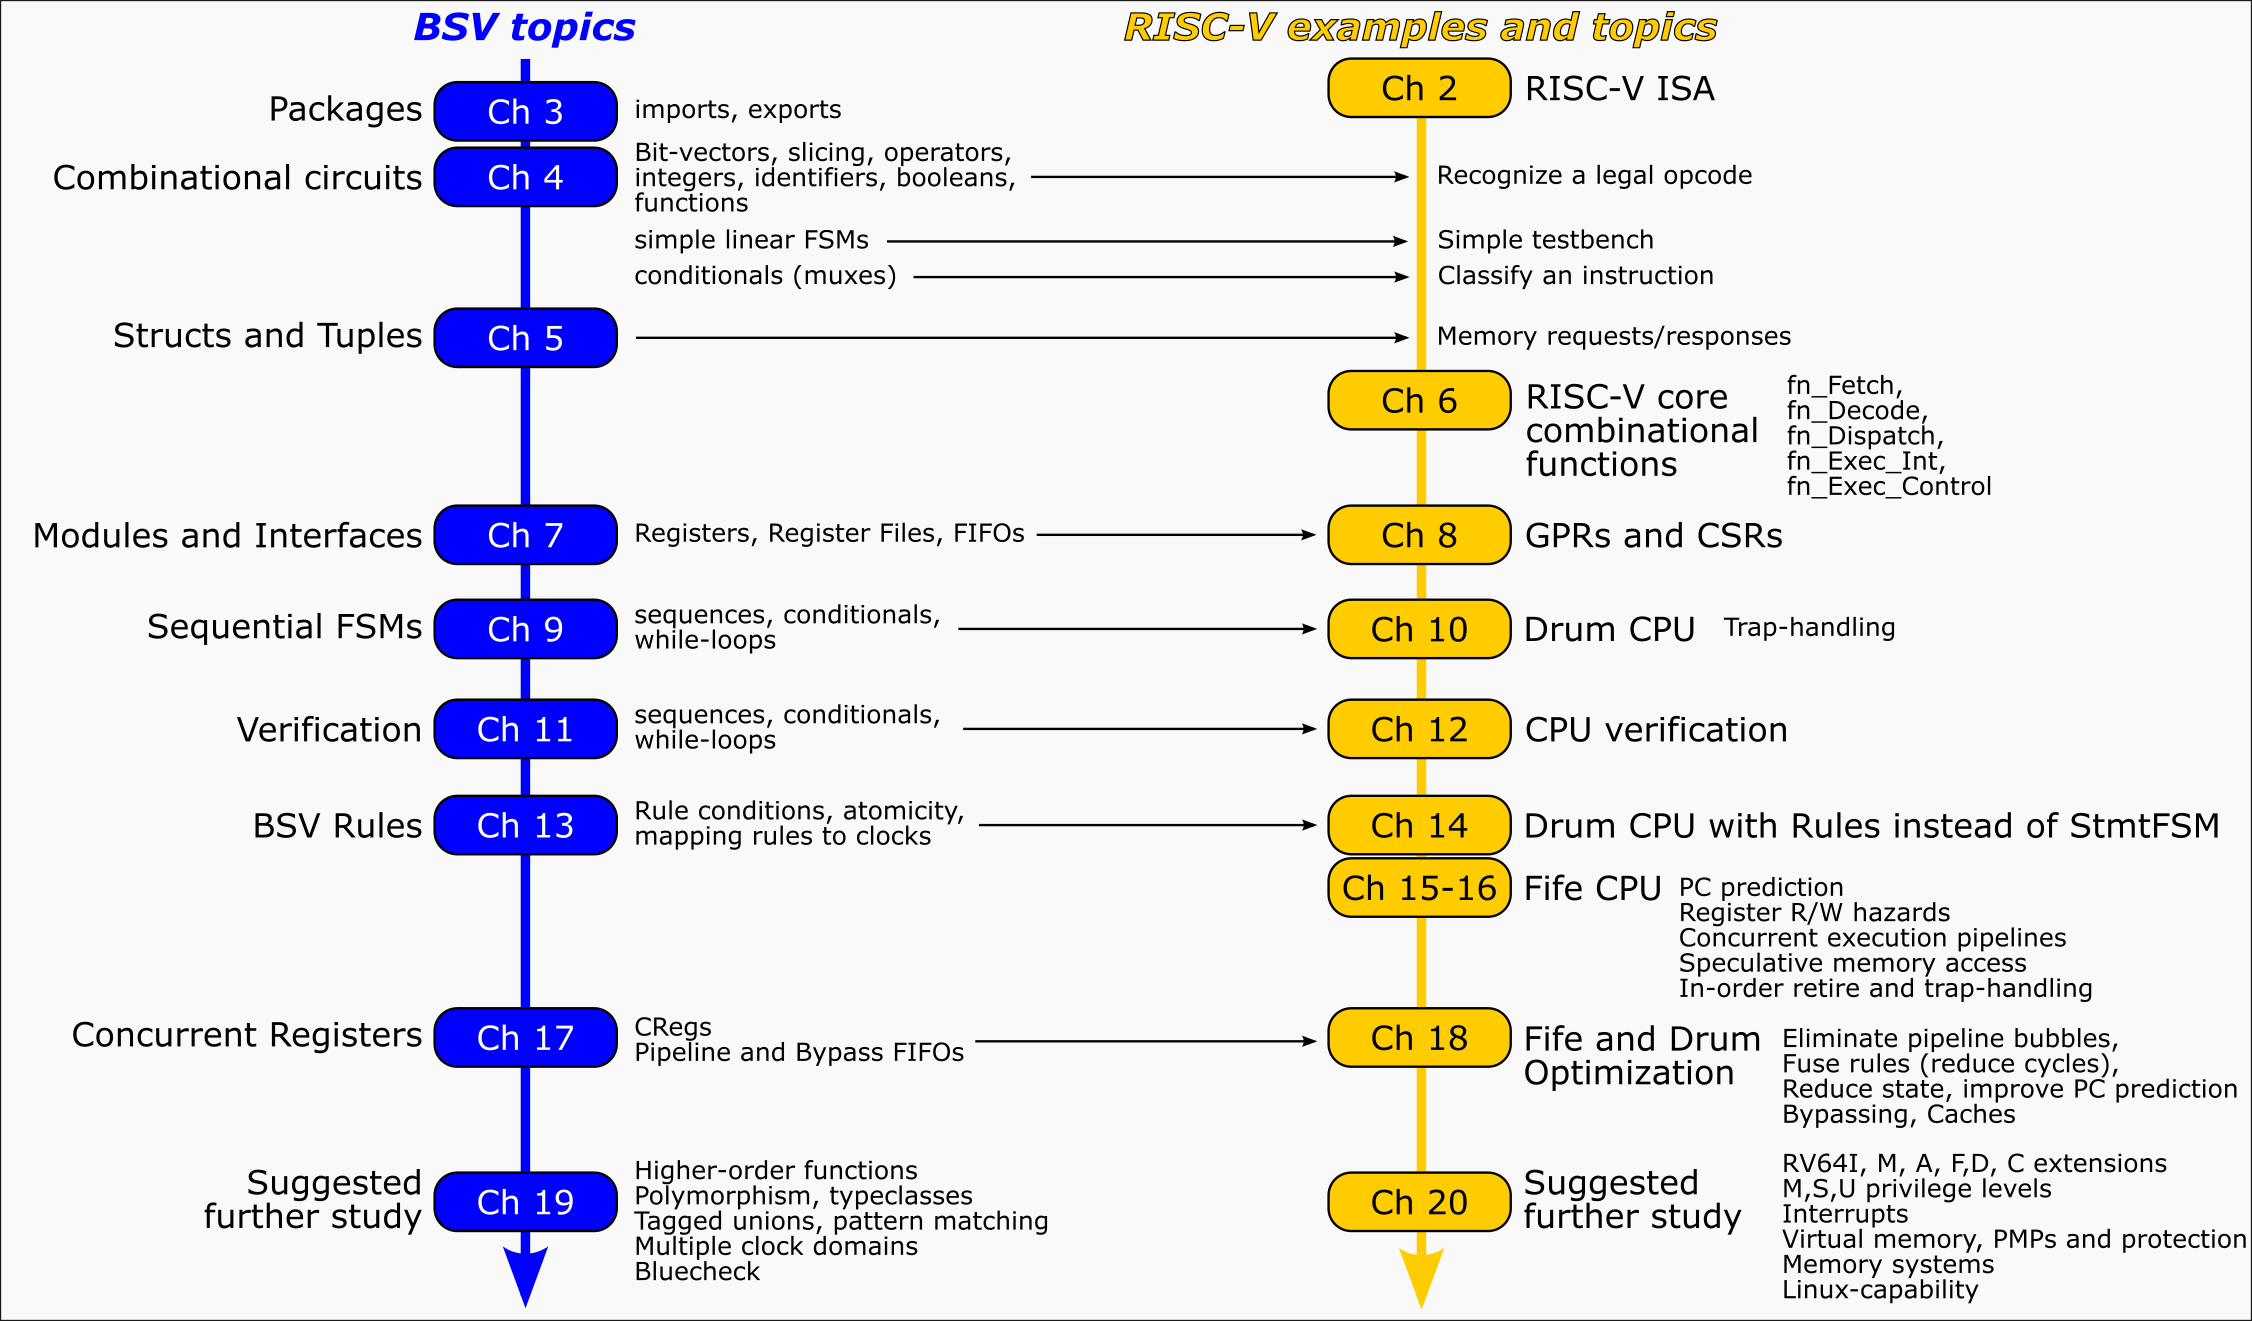
\includegraphics[height=0.825\textheight]{Fig_Chapter_Roadmap}}
\end{center}

\end{frame}

% ================================================================


% ================================================================

\begin{frame}
\frametitle{Table of Contents}

\tableofcontents

\end{frame}

% ****************************************************************

\section{Motivation}

\begin{frame}

\begin{center}
  {\LARGE BSV: Tighter Rule Scheduling: Motivation}
\end{center}

\end{frame}

% ================================================================

\begin{frame}[fragile]
\frametitle{Tighter Rule Scheduling: Motivation}

\footnotesize

\begin{tabular}{ | c | p{0.55\textwidth} | p{0.35\textwidth} | }
 \hline
   \hm & {\BSV} & \scriptsize \emph{Analogy: RISC-V ISA} \\
 \hline
 \hline
     (A)

   & Rule semantics are abstract: one rule at a time

   & \scriptsize \emph{RISC-V ISA semantics are abstract: one instruction at a time}

   \\

 \hline
     (B)

   & When the {\bsc} compiler maps a set of rules to execute
     simultaneously (in the same clock), all their methods occur at
     the same instant (clock edge). All ``read-values'' are from the
     previous clock edge; all ``write-values'' ({\tt Action} and {\tt
     ActionValue} results) are visible only at the next clock edge.

     \vspace{1ex}

     {\bsc} must ensure that the \emph{ordering} of methods in (B) is
     consistent with (A).

     \vspace{1ex}

     In particular, {\bsc} may introduce (combinational) control
     circuits to \emph{stall} a rule to avoid violating (A).

   & \scriptsize

     \emph{RISC-V instructions can be executed in pipelines, in parallel
     (superscalar), out-of-order, ...  The implementation must ensure
     that the \emph{order} in which they retire, and the \emph{order} in
     which they read and write registers and memory, is consistent
     with (A).

     \vspace{1ex}

     In particular, an instruction may be \emph{stalled} to avoid
     violating (A).}

   \\
 \hline
\end{tabular}

\end{frame}

% ================================================================

\subsection{Motivational Example}

\begin{frame}[fragile]
\frametitle{Tighter Rule Scheduling: Motivational Example: Up-Down Counter (1/2)}

\footnotesize

Consider this scenario, where a Producer streams packets over a long
connection to a Consumer:

\begin{center}
 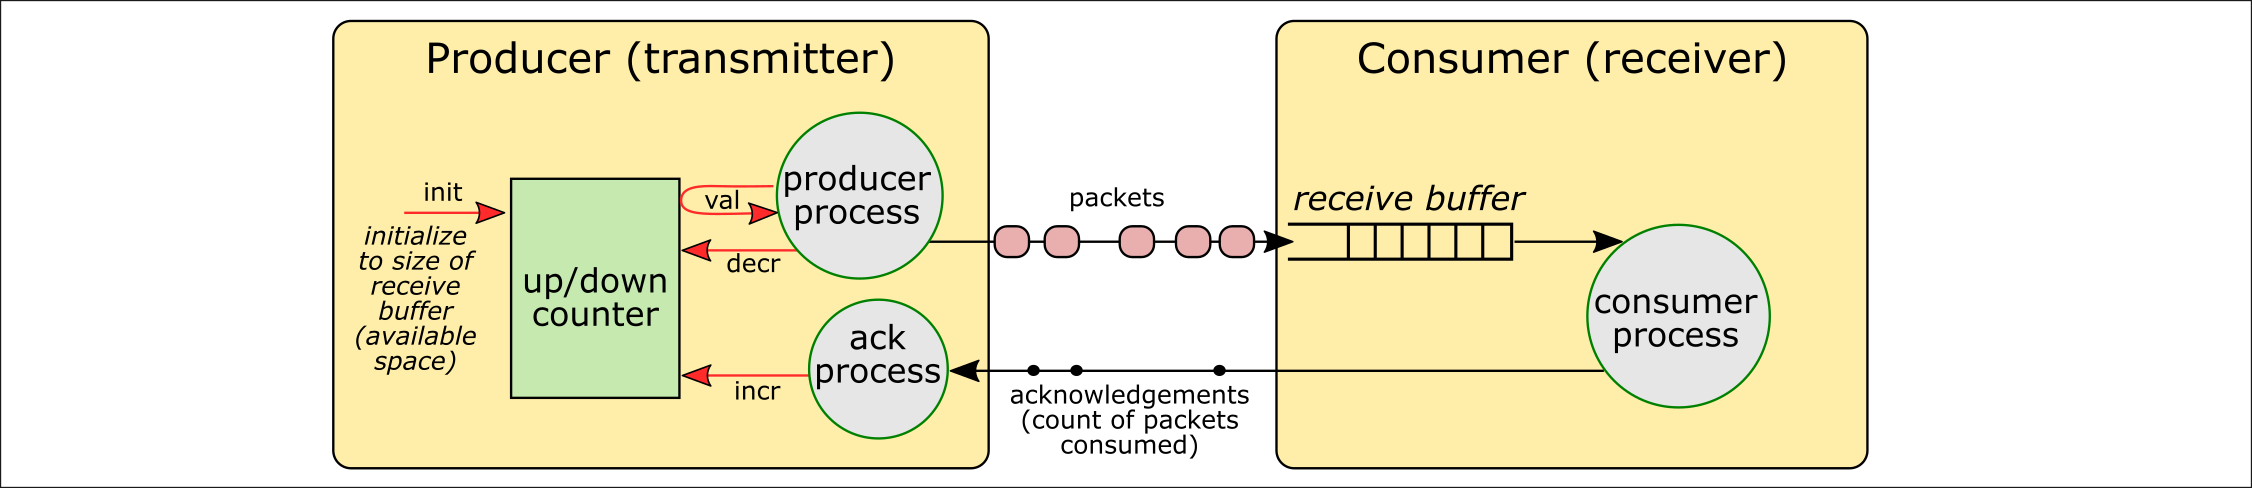
\includegraphics[width=0.9\textwidth]{Fig_Credit_Based_Flow_Control}
\end{center}

\begin{minipage}{0.38\textwidth}\scriptsize
\begin{Verbatim}[frame=single]
interface Up_Down_Counter_IFC;
   method Action   init (Bit #(4) init_val);
   method Bit #(4) val;
   method Action   decr;
   method Action   incr;
endinterface
\end{Verbatim}
\end{minipage}
\begin{minipage}{0.6\textwidth}

To avoid over-running the receive buffer,   The producer:

\begin{itemize}
 \item initializes the counter to the available space in the buffer;
 \item for every packet sent, decrements the counter  ({\tt decr} method);
 \item stalls (doesn't send) if the counter value ({\tt val} method) is zero (no space available).
\end{itemize}

As the receiver consumes packets from the buffer, it sends
acknowledgements back to indicate the amount of space freed.

\vspace{1ex}

In the transmitter, acknowledgements are incremented back into the
counter ({\tt incr} method), allowing transmission to continue.
\end{minipage}

\end{frame}

% ----------------------------------------------------------------

\begin{frame}[fragile]
\frametitle{Tighter Rule Scheduling: Motivational Example: Up-Down Counter (2/2)}

\footnotesize

Here is a possible implementation of the ``Up-Down'' Counter:

\begin{minipage}{0.45\textwidth}\scriptsize
\begin{Verbatim}[frame=single]
module mkUp_Down_Counter_I (Up_Down_Counter_IFC);
   // STATE
   Reg #(Bit #(4)) rg_counter <- mkReg (15);

   // --------------------------------
   // INTERFACE

   method Action init (Bit #(4) init_val);
      rg_counter <= init_val;
   endmethod

   method Bit #(4) val;
      return rg_counter;
   endmethod

   method Action decr () if (rg_counter != 0);
      rg_counter <= rg_counter - 1;
   endmethod

   method Action incr () if (rg_counter != 15);
      rg_counter <= rg_counter + 1;
   endmethod
endmodule
\end{Verbatim}
\end{minipage}
\hm
\begin{minipage}{0.5\textwidth}

Analysis: Rules invoking {\tt .incr()} and {\tt .decr()} cannot execute on the same clock edge.

\begin{itemize}\scriptsize

 \item (A) In the abstract rule semantics, either {\tt .incr()}
       precedes {\tt .decr()} or \emph{vice versa}.

       \vspace{1ex}

       In either case, the latter rule observes the update from the previous rule.

       \vspace{2ex}

 \item (B) If they executed on the same clock, neither rule sees the
       update from the other rule.  This is inconsistent with (A).

\end{itemize}

\vspace{1ex}

{\scriptsize
Thus, this implementation cannot send a packet (decr) and
register an ack (incr) in the same clock, even though the two streams
are asynchronous and concurrent.}

\vspace{1ex}

{\scriptsize
On the average, we can only send (and register ack) on every alternate clock.}

\vspace{3ex}

{\bf Solution:} \\
Use a \emph{Concurrent Register} ({\tt CReg}) for {\tt rg\_counter}.

\end{minipage}

\end{frame}

% ****************************************************************

\section{Concurrent Registers}

\begin{frame}

\begin{center}
  {\LARGE BSV: Concurrent Registers ({\tt CReg}s)}
\end{center}

\end{frame}

% ================================================================

\subsection{CRegs}

\begin{frame}[fragile]
\frametitle{CRegs}

\footnotesize

A Concurrent Register, or \verb|CReg|, is a module provided by
 the \emph{bsc} library.  Its interface is an \emph{array}
 of \verb|Reg#(t)| interfaces:

\begin{Verbatim}[frame=single]
module mkCReg #(parameter Integer n,
                parameter a_type resetval)
              (Reg#(a_type) ifc[])
\end{Verbatim}

\vspace{5ex}

It is instantiated similar to this example: \\
(This example: register content type: \verb|Bit#(4)|; initial value: 15; two {\tt Reg} interfaces).

\begin{Verbatim}[frame=single]
   // parameter n is 2, resetval is 15
   Array #(Reg #(Bit #(4))) crg_counter <- mkCReg (2, 15);
\end{Verbatim}

\end{frame}

% ================================================================

\subsection{Hardware intuition}

\begin{frame}[fragile]
\frametitle{Hardware intuition for a CReg}

\label{slide_hw_intuition}

\footnotesize

\begin{center}
 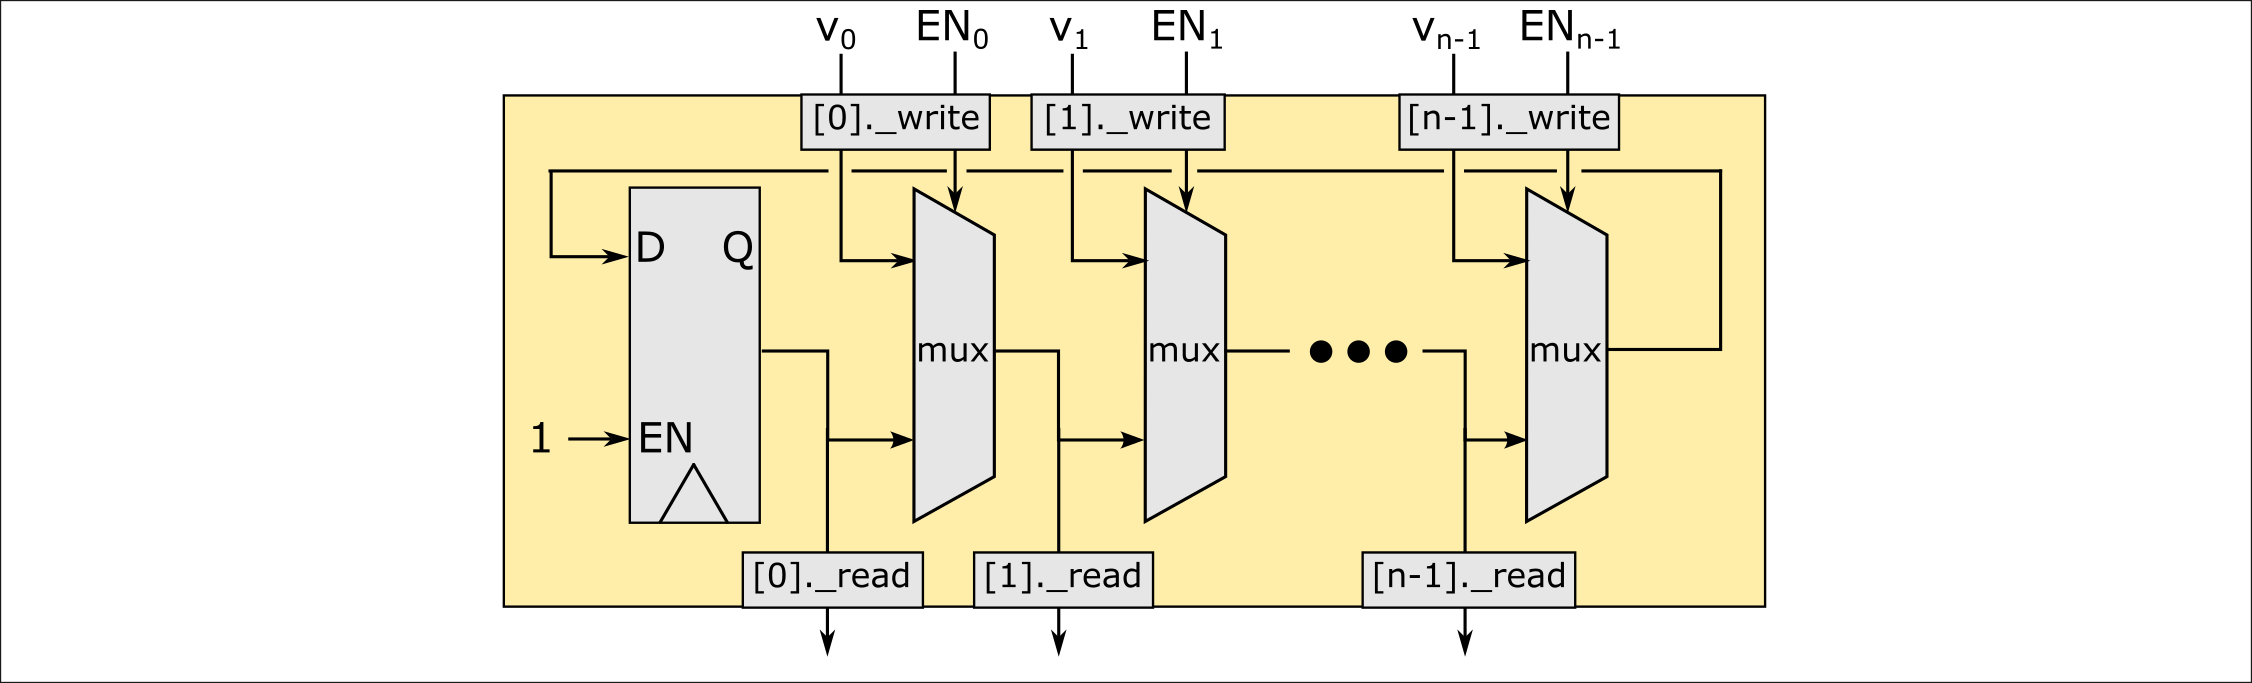
\includegraphics[width=\textwidth]{Fig_CReg_HW}

 \vspace{1ex}

 This has an array of $n$ {\tt Reg} interfaces, indexed from 0 to $n$-1.

 \vspace{1ex}

 The $j$'th interface has {\tt [$j$].\_read()} and {\tt [$j$].\_write()} methods.
\end{center}

\end{frame}

% ================================================================

\subsection{CReg ordering properties}

\begin{frame}[fragile]
\frametitle{CReg ordering properties}

\footnotesize

\fbox{
\begin{minipage}{0.6\textwidth}
\begin{itemize}

 \item All the methods can be invoked in the same clock.

 \item A read at the $j$'th register interface,{\ie} {\tt x[$j$].\_read}
       returns the latest of:

       \begin{itemize}\footnotesize
        \item the value $v_{j-1}$, if {\tt x[$j-1$].\_write($v_{j-1}$)} is being invoked;
        \item else the value $v_{j-2}$, if {\tt x[$j-2$].\_write($v_{j-2}$)} is being invoked;
        \item ...
        \item else the value $v_1$, if {\tt x[1].\_write($v_1$)} is being invoked;
        \item else the value $v_0$, if {\tt x[0].\_write($v_0$)} is being invoked;
        \item else the value in the register.
       \end{itemize}

 \item The register value is updated with the latest of:

       \begin{itemize}\footnotesize
        \item the value $v_{n-1}$, if {\tt x[$n-1$].\_write($v_{n-1}$)} is being invoked;
        \item else the value $v_{n-2}$, if {\tt x[$n-2$].\_write($v_{n-2}$)} is being invoked;
        \item ...
        \item else the value $v_1$, if {\tt x[1].\_write($v_1$)} is being invoked;
        \item else the value $v_0$, if {\tt x[0].\_write($v_0$)} is being invoked;
        \item else the current value in the register.
       \end{itemize}

\end{itemize}
\end{minipage}}
\hm
\begin{minipage}{0.35\textwidth}

This ordering corresponds exactly to the left-to-right and
top-to-bottom ordering of the methods in the hardware-intuition
diagram (Slide~\ref{slide_hw_intuition}).

\end{minipage}

\end{frame}

% ================================================================

\subsection{Up-down counter with CReg}

\begin{frame}[fragile]
\frametitle{Up-down counter with a CReg}

\footnotesize

\begin{minipage}{0.5\textwidth}\scriptsize
\begin{Verbatim}[frame=single]
module mkUp_Down_Counter_I (Up_Down_Counter_IFC);
   // STATE
   Array #(Reg #(Bit #(4))) crg_counter <- mkCReg (3,15);

   // --------------------------------
   // INTERFACE
   method Action init (Bit #(4) init_val);
      crg_counter [2] <= init_val
   endmethod

   method Bit #(4) val;
      return rg_counter [0];
   endmethod

   method Action decr if (rg_counter != 0);
      rg_counter [1] <= rg_counter [1] - 1;
   endmethod

   method Action incr if (rg_counter != 15);
      rg_counter [0] <= rg_counter [0] + 1;
   endmethod
endmodule
\end{Verbatim}
\end{minipage}
\hm
\begin{minipage}{0.45\textwidth}
 Some questions to ponder:

 \begin{itemize}

  \item What does method {\tt val} return? \\
        \hm The original value in the register? \\
        \hm The value after the increment? \\
        \hm The value after the decrement? \\
        \hm The value after the increment and decrement?

  \item What happens if methods {\tt incr} and {\tt decr} are called
        simultaneously?  Which one happens (semantically) ``first''?

        Note: {\tt incr} saturates at 15, and {\tt decr} saturates at
        0, so the order matters!

 \end{itemize}

 \vspace{2ex}

 \emph{Hint:} The answers are in the choice of {\tt CReg} indexes in each method.
\end{minipage}

\end{frame}

% ================================================================

\subsection{Example: CSR {\tt mcycle} in RISC-V}

\begin{frame}[fragile]
\frametitle{Example: CSR {\tt mcycle} in RISC-V}

\footnotesize

CSR {\tt mcycle} (RISC-V CPU cycle counter) is updated by two ``processes'':

\begin{itemize}

 \item (A) Standalone infinite loop incrementing {\tt mcycle} on every cycle.

 \item (B) Instruction execution, when we have a {\tt CSRRxx} instruction
           that writes to {\tt mcycle}.
\end{itemize}

The RISC-V spec says that when (B) happens, it should override (A).

\PAUSE{\vspace{5ex}}

We can instantiate a CReg for this:

\vspace{1ex}

\begin{Verbatim}[frame=single, label=from src\_Common/CSRs.bsv]
   Array #(Reg #(Bit #(64))) csr_mcycle <- mkCReg (2, 0);
\end{Verbatim}

\vspace{2ex}

(A) Standalone process incrementing it:

\vspace{1ex}

\begin{Verbatim}[frame=single, label=from src\_Common/CSRs.bsv]
   rule rl_count_cycles;
      csr_mcycle [0] <= csr_mcycle [0] + 1;
   endrule
\end{Verbatim}

\vspace{2ex}

(B) CSRRxx instruction execution (overrides (A) because of higher CReg index):

\vspace{1ex}

\begin{Verbatim}[frame=single, label=from src\_Common/CSRs.bsv in function fav\_csr\_write()]
   csr_mcycle [1] <= csr_val;
\end{Verbatim}

\end{frame}

% ****************************************************************

\section{SpecialFIFOFs}

\begin{frame}

\begin{center}
  {\LARGE BSV: Higher-performance FIFOs (in library {\tt SpecialFIFOs})}

  \vspace{5ex}

  (implemented using Concurrent Registers)
\end{center}

\end{frame}

% ================================================================

\begin{frame}[fragile]
\frametitle{A FIFO implemented with ordinary registers}

\footnotesize

Consider the following module implementing a 1-element FIFO with a
FIFOF interface, \\
using ordinary registers ({\tt mkReg}, {\tt mkRegU}):

\vspace{2ex}

\begin{center}
\begin{minipage}[t]{0.45\textwidth}\scriptsize
\begin{Verbatim}[frame=single]
module mkFIFOF (FIFOF #(Bit #(32)));
   Reg #(Bit #(32)) rg_data <- mkRegU;
   Reg #(Bool)      rg_full <- mkReg (False);

   // ----------------
   // INTERFACE

   method Bool notEmpty ();
      return rg_full;
   endmethod

   method Bit #(32) first () if (rg_full);
      return rg_data;
   endmethod

   method Action deq () if (rg_full);
      rg_full <= False;
   endmethod
   ...
\end{Verbatim}
\end{minipage}
\begin{minipage}[t]{0.45\textwidth}\scriptsize
\begin{Verbatim}[frame=single]
   ...
   method Bool notFull ();
      return (! rg_full);
   endmethod

   method Action enq (Bit #(32) x) if (! rg_full);
      rg_data <= x;
      rg_full <= True;
   endmethod

   method Action clear;
      rg_full <= False;
   endmethod
endmodule
\end{Verbatim}
\end{minipage}
\end{center}

\end{frame}

% ================================================================

\begin{frame}[fragile]
\frametitle{Analysis of the performance of {\tt mkFIFOF}}

\footnotesize

Consider a producer rule \verb|rl_P| that invokes \verb|enq|, and a
consumer rule \verb|rl_C| that invokes \verb|first| and \verb|deq|:

\vspace{4ex}

\begin{center}
 
\includegraphics[width=\textwidth]{Fig_FIFO_Producer_Consumer}
\end{center}

\vspace{4ex}

These rules cannot fire at the same instant (on the same clock)
because both of them read and write register \verb|fg_Full| (because
both \verb|enq| and \verb|deq| read and write the register).

\vspace{2ex}

We can use a CReg to relax this constraint, in two different ways,
which we call {\tt mkPipelineFIFOF} and {\tt mkBypassFIFOF},
respectively.

\end{frame}

% ================================================================

\subsection{PipelineFIFOs}

\begin{frame}[fragile]
\frametitle{{\tt mkPipelineFIFOF}}

\label{mkPipelineFIFOF}

\footnotesize

Instead of {\tt mkReg} for {\tt rg\_full}, we can use {\tt mkCReg}:

\begin{center}
\begin{minipage}[t]{0.485\textwidth}\scriptsize
\begin{Verbatim}[frame=single]
module mkFIFOF (FIFOF #(Bit #(32)));
module mkPipelineFIFOF (FIFOF #(Bit #(32)))
   Reg #(Bit #(t))      rg_data  <- mkRegU;
   Array #(Reg #(Bool)) crg_full <- mkCReg (3, False);

   // ----------------
   // INTERFACE

   method Bool notEmpty ();
      return crg_full [0];
   endmethod

   method Bit #(32) first () if (crg_full [0]);
      return rg_data;
   endmethod

   method Action deq () if (crg_full [0]);
      crg_full [0] <= False;
   endmethod
   ...
\end{Verbatim}
\end{minipage}
\begin{minipage}[t]{0.485\textwidth}\scriptsize
\begin{Verbatim}[frame=single]
   ...
   method Bool notFull ();
      return (! crg_full [1]);
   endmethod

   method Action enq (Bit #(32) x) if (! crg_full [1]);
      rg_data      <= x;
      crg_full [1] <= True;
   endmethod

   method Action clear;
      crg_full [2] <= False;
   endmethod
endmodule
\end{Verbatim}

\vspace{1ex}

Note that the ``dequeue'' side methods use index [0], ``enqueue'' side
use methods index [1]; and ``clear'' uses index [2].

\vspace{1ex}

These choices affect the ordering semantics of the methods.

\end{minipage}
\end{center}

\end{frame}

% ================================================================

\begin{frame}[fragile]
\frametitle{Analysis of the performance of {\tt mkPipelineFIFOF}}

\footnotesize

\begin{minipage}{0.45\textwidth}
  Consider again a producer rule \verb|rl_P| that invokes \verb|enq|, and a
  consumer rule \verb|rl_C| that invokes \verb|first| and \verb|deq|:
\end{minipage}
\hm
\begin{minipage}{0.5\textwidth}
  
\includegraphics[width=\textwidth]{Fig_FIFO_Producer_Consumer}
\end{minipage}

\vspace{5ex}

Because of {\tt mkPipelineFIFOF}'s CReg indexes, in the equivalent
rule-at-a-time semantics, \verb|rl_C| fires \emph{before} \verb|rl_P|.
Thus, even if the FIFO was full at the start of the clock, \verb|rl_P|
can still \verb|enq| into the FIFO, \emph{provided} \verb|rl_C| is
firing on the same clock.

\vspace{1ex}

Per the rule-at-a-time semantics,
\verb|rl_C| fires first, which empties the FIFO, {\ie} \verb|rl_P|
sees the FIFO as empty and is therefore able to \verb|enq| into it.

\vspace{1ex}

This is why we call it a ``PipelineFIFO'': it is an ideal candidate
for the FIFO between stages of a pipeline, allowing the downstreanm
stage (the consumer) and the upstream stage (the producer) to fire on
the same clock, advancing data in a piplined manner.

\vspace{2ex}

Note also that another rule invoking \verb|clear|, too, can fire on
the same clock as \verb|rl_P| and \verb|rl_C|.  Because of its CReg
index, logically it fires ``last'', and so will leave the FIFO in a
finally empty state.

\end{frame}

% ================================================================

\begin{frame}[fragile]
\frametitle{Analysis of the hardware for {\tt mkPipelineFIFOF}}

\footnotesize

In the Verilog for \verb|mkPipelineFIFOF|, the READY signal
for \verb|enq| incorporates the ENABLE signal of the \verb|deq| method
(because if the FIFO is full from the previous clock, in this
clock \verb|enq| can only be invoked if \verb|deq| is also being
invoked).

\vspace{2ex}

Thus, there is a \emph{combinational path} backward through the FIFO
(a path that involves only wires and gates and no state-element) from
the \verb|deq| method to the \verb|enq| method.

\vspace{2ex}

\begin{center}
  \includegraphics[width=\textwidth]{Fig_Combo_path_in_mkPipelineFIFOF}
\end{center}

\end{frame}

% ================================================================

\subsection{BypassFIFOs}

\begin{frame}[fragile]
\frametitle{{\tt mkBypassFIFOF}}

\label{mkBypassFIFOF}

\footnotesize

What happens if we exchange the [0] and [1] CReg indexes?

\begin{center}
\begin{minipage}[t]{0.485\textwidth}\scriptsize
\begin{Verbatim}[frame=single]
   Array #(Reg #(Bit #(32))) crg_data <- mkCRegU (2);
   Array #(Reg #(Bool))      crg_full <- mkCReg (3, False);

   // ----------------
   // INTERFACE

   method Bool notEmpty ();
      return crg_full [1];
   endmethod

   method Bit #(32) first () if (crg_full [1]);
      return crg_data [1];
   endmethod

   method Action deq () if (crg_full [1]);
      crg_full [1] <= False;
   endmethod
   ...
\end{Verbatim}
\end{minipage}
\begin{minipage}[t]{0.485\textwidth}\scriptsize
\begin{Verbatim}[frame=single]
   ...
   method Bool notFull ();
      return (! crg_full [0]);
   endmethod

   method Action enq (Bit #(32) x) if (! crg_full [0]);
      crg_data [0] <= x;
      crg_full [0] <= True;
   endmethod

   method Action clear;
      crg_full [0] <= False;
   endmethod
endmodule
\end{Verbatim}

\vspace{1ex}

Now, the ``enqueue'' side methods use index [0] and the ``dequeue''
side methods use index [1] (``clear'' still uses index [2]).

\vspace{1ex}

These choices change the ordering semantics of the methods.

\end{minipage}
\end{center}

\end{frame}

% ================================================================

\begin{frame}[fragile]
\frametitle{Analysis of the performance of {\tt mkBypassFIFOF}}

\footnotesize

\begin{minipage}{0.45\textwidth}
  Consider again a producer rule \verb|rl_P| that invokes \verb|enq|, and a
  consumer rule \verb|rl_C| that invokes \verb|first| and \verb|deq|:
\end{minipage}
\hm
\begin{minipage}{0.5\textwidth}
  
\includegraphics[width=\textwidth]{Fig_FIFO_Producer_Consumer}
\end{minipage}

\vspace{5ex}

Because of {\tt mkBypassFIFOF}'s CReg indexes, in the equivalent
rule-at-a-time semantics, \verb|rl_C| fires \emph{after} \verb|rl_P|.
Thus, even if the FIFO was empty at the start of the clock, \verb|rl_C|
can still \verb|deq| from the FIFO, \emph{provided} \verb|rl_P| is
firing on the same clock.

\vspace{1ex}

Per the rule-at-a-time semantics, \verb|rl_P| fires first, which fills
the empty FIFO, {\ie} \verb|rl_C| sees the FIFO as full and is
therefore able to \verb|deq| from it.

\vspace{1ex}

This is why we call it a ``BypassFIFO''.  When used in a pipeline, the
enqueued value can be ``bypassed'' straight through the FIFO to the
consumer on the same clock.

\vspace{2ex}

As with {\tt mkPipelineFIFOF}, another rule invoking \verb|clear|,
too, can fire on the same clock as \verb|rl_P| and \verb|rl_C|.
Because of its CReg index, logically it fires ``last'', and so will
leave the FIFO in a finally empty state.

\end{frame}

% ================================================================

\begin{frame}[fragile]
\frametitle{Analysis of the hardware for {\tt mkBypassFIFOF}}

\footnotesize

In the Verilog for \verb|mkBypassFIFOF|, the READY signal
for \verb|first| and \verb|deq| incorporates the ENABLE signal of
the \verb|enq| method (because if the FIFO is empty from the previous
clock, in this clock \verb|first| and \verb|deq| can only be invoked
if \verb|enq| is also being invoked).

\vspace{2ex}

Similarly, for the data to be bypassed through, there has to be a
combinational path from the \verb|enq| argument to the \verb|first|
result.

\vspace{2ex}

Thus, there are \emph{combinational paths} forward through the FIFO
(paths that involve only wires and gates and no state-element) from
the \verb|enq| method to the \verb|first| and \verb|deq| methods.

\vspace{2ex}

\begin{center}
  \includegraphics[width=\textwidth]{Fig_Combo_path_in_mkBypassFIFOF}
\end{center}

\end{frame}

% ================================================================

\begin{frame}

\frametitle{Summary of {\tt mkFIFOF}, {\tt mkPipelineFIFOF} and {\tt mkBypassFIFOF}}

\footnotesize

\begin{center}
    \begin{tabular}{|l|c|c|c|}
      \hline
          &
          {\tt mkFIFOF} &
          {\tt mkPipelineFIFOF} &
          {\tt mkBypassFIFOF} \\
      \hline
      \hline
        1-tick traversal       &   Yes   &  Yes  &  Yes  \\
      \hline
        \# of buffer registers &    2    &   1   &   1   \\
      \hline
        Scheduling constraints &
        None &
        {\tt deq} before {\tt enq} &
        {\tt enq} before {\tt deq} \\
      \hline
        Through combinational circuits &
        None &
        {\tt deq} $\rightarrow$ {\tt enq} &
        {\tt enq} $\rightarrow$ {\tt deq} \\
      \hline
        Separate compilation of stages &
        No &
        No &
        No \\
      \hline
    \end{tabular}
\end{center}

\vx

In the next section we'll discuss an alternative: back-to-back
composition of {\tt mkBypassFIFOF} and {\tt mkPipelineFIFOF}

\end{frame}

% ****************************************************************

\section{Connecting Pipeline Stages}

\begin{frame}

\begin{center}
  {\LARGE BSV: Connecting pipeline stages}
\end{center}

\end{frame}

% ================================================================

\subsection{Back-to-back BypassFIFO+PipelineFIFO}

\begin{frame}[fragile]
\frametitle{Back-to-back composition of BypassFIFO and PipelineFIFO (1/2)}

\label{slide_back_to_back_fifos}

\footnotesize

\begin{minipage}{0.5\textwidth}
An interesting component is a back-to-back composition of the two
high-performance FIFOs we have discussed.

\vspace{2ex}

Consider this code fragment, illustrated below:

\vspace{5ex}

\begin{center}
  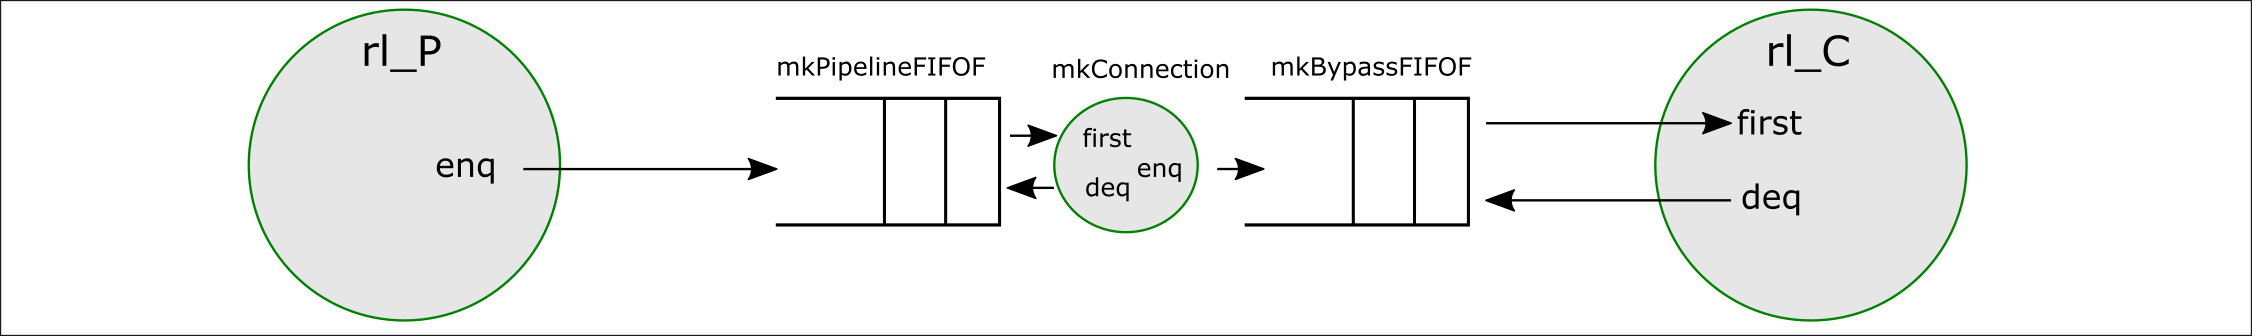
\includegraphics[width=\textwidth]{Fig_Composed_FIFO_Producer_Consumer}
\end{center}


\end{minipage}
\hm
\begin{minipage}{0.47\textwidth}\scriptsize
\begin{Verbatim}[frame=single]
module mk... (...);
   FIFOF #(Bit #(32)) f_bypass   <- mkBypassFIFOF;
   FIFOF #(Bit #(32)) f_pipeline <- mkPipelineFIFOF;

   // Producer rule (into f_bypass's enq side)
   rule rl_P;
      ... f_bypass.enq (x);
   endrule

   // Connect f_bypass's first/deq side
   // to f_pipeline's enq side
   mkConnection (to_FIFO_O (f_bypass),
                 to_FIFO_I (f_pipeline));

   // Consumer rule (from f_pipeline's first/deq side)
   rule rl_C;
      let y = f_pipeline.first;
      f_pipeline.deq;
   endrule
endmodule
\end{Verbatim}
\end{minipage}

\end{frame}

% ================================================================

\begin{frame}[fragile]
\frametitle{Back-to-back composition of BypassFIFO and PipelineFIFO (2/2)}

\label{Slide_FIFO_Composition}

\footnotesize

This has some pleasant properties:

\vspace{1ex}

\begin{itemize}

 \item Despite there being two FIFOs, it takes only one tick to
        traverse them (because of the nature of BypassFIFOs).

 \PAUSE{\vx}

 \item There are no ordering constraints across the composed FIFOs,
       {\ie} the FIFOs do not induce any ordering constraints between
       the producer rule \verb|rl_P| and the consumer rule \verb|rl_C|
       (they are ``conflict free'').  They can fire in the same clock
       and can go in either logical order.

 \PAUSE{\vx}

 \item There are no combinational paths through the pair of FIFOs!
       One can verify this by studying the Verilog.  The \emph{bsc}
       compiler also helpfully reports the absence of combinational
       paths.

 \PAUSE{\vx}

 \item Enables easier separate compilation (into Verilog) of stage
       modules: place one of the two component FIFOs in each stage
       module, and use {\tt mkConnection} in the parent module.

       \vx

       (Separate compilation is possible with the other FIFOs, but is messier.)

\end{itemize}

\PAUSE{\vxxxx}

\begin{minipage}{0.37\textwidth}
This makes it attractive for connecting stages in a pipeline, enabling
a \emph{modular} separation of stages, where each stage can be
independently verified and compiled to Verilog. We use this technique
everywhere in Fife.
\end{minipage}
\hfill
\begin{minipage}{0.6\textwidth}
  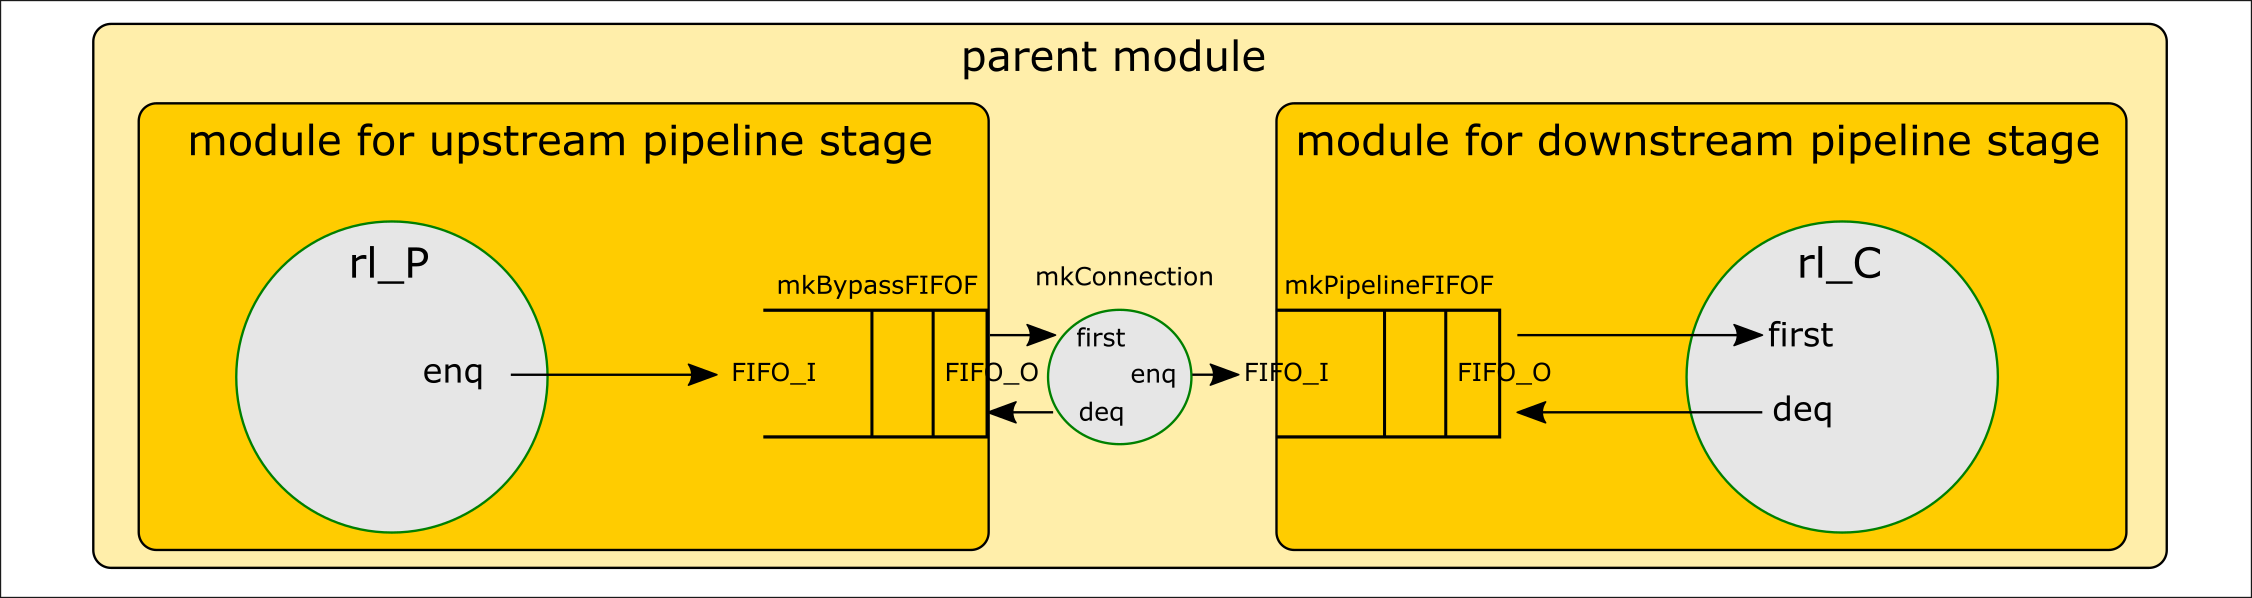
\includegraphics[width=\textwidth]{Fig_Composed_FIFO_modularity}
\end{minipage}

\end{frame}

% ================================================================

\begin{frame}

\frametitle{Summary of {\tt mkPipelineFIFOF} and {\tt mkBypassFIFOF} and their composition}

\footnotesize

\begin{center}
    \begin{tabular}{|l|c|c|c|c|}
      \hline
          &
          {\tt mkFIFOF} &
          {\tt mkPipelineFIFOF} &
          {\tt mkBypassFIFOF} &
          Composition \\
      \hline
      \hline
        1-tick traversal       &   Yes   &  Yes  &  Yes  & Yes \\
      \hline
        \# of buffer registers &    2    &   1   &   1   &  2 \\
      \hline
        Scheduling constraints &
        None &
        {\tt deq} before {\tt enq} &
        {\tt enq} before {\tt deq} &
        None \\
      \hline
        Through combinational circuits &
        None &
        {\tt deq} $\rightarrow$ {\tt enq} &
        {\tt enq} $\rightarrow$ {\tt deq} &
        None  \\
      \hline
        Separate compilation of stages &
        No &
        No &
        No &
        Yes  \\
      \hline
    \end{tabular}
\end{center}

\end{frame}

% ****************************************************************

\section{Final Comments}

\begin{frame}[fragile]
\frametitle{Final comments on CRegs}

\footnotesize

\begin{itemize}

 \item CRegs allow us to save a cycle by allowing two rules to run
       concurrently in the same clock where previously they had to run
       in separate clocks.

       \vspace{1ex}

       Effectively, CRegs allow us safely to \emph{fuse} the actions
       in two different rules into a single composite action (whenever
       the rule conditions allow)

 \item It plays a central rule in fine-tuning {\BSV} designs for
       optimal performance, without changing the functional semantics
       (rule-at-a-time).

       \vspace{1ex}

       In RISC-V designs, CRegs enable:
       \begin{itemize}\footnotesize

         \item Isolation of stages (no combinational paths) while
               preserving pipeline speed (as discussed in
               Slide~\ref{Slide_FIFO_Composition}).

         \item Faster PC redirection after a misprediction
         \item Faster resolution of register dependencies in the scoreboard
         \item Faster reorder buffers in Out-Of-Order processors
         \item ... and more ...
       \end{itemize}

\end{itemize}

\PAUSE{\vspace*{5ex}}

 \emph{Caveat: Before CRegs were available in {\BSV}, designs used a
       facility called ``RWires'' for the same fusion optimizations.
       RWires are still available in BSV (see library documentation),
       but we recommend using CRegs in new designs.  RWires muddy the
       otherwise clear separation of functional semantics (logical)
       and clocked semantics (implementation).}

\end{frame}

% ****************************************************************

% -*- mode: fundamental -*-

% Slides accompanying "Learn RISC-V CPU Implementation and BSV" book
% Copyright (c) 2024 Rishiyur S. Nikhil, All Rights Reserved

% This is a postamble shared by all the slide decks

% ================================================================

\begin{frame}

\begin{center}
  {\LARGE End}
\end{center}

\end{frame}

% ================================================================


% ****************************************************************

\end{document}

% ****************************************************************
